\renewcommand{\thesection}{\Alph{section}}

\begin{appendices}
\chapter{Appendix}

\section{\ac{epc} Schemes and Corresponding GS1 keys} \label{anx:epccodingschemes}
\begin{table}[!ht]
    \centering
    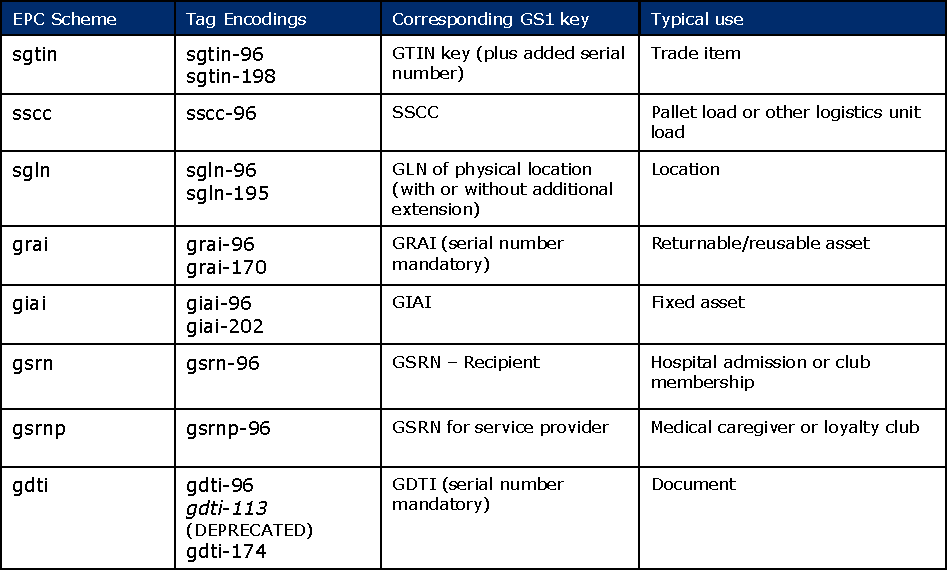
\includegraphics[width=\textwidth]{./figs/02-state-of-the-art/epcschemes.pdf}
    \caption[\ac{epc} Schemes and Corresponding GS1 keys Part 1]{\ac{epc} Schemes and Corresponding GS1 keys Part 1~\cite{EPCTagData}}
\end{table}

\begin{table}
    \centering
    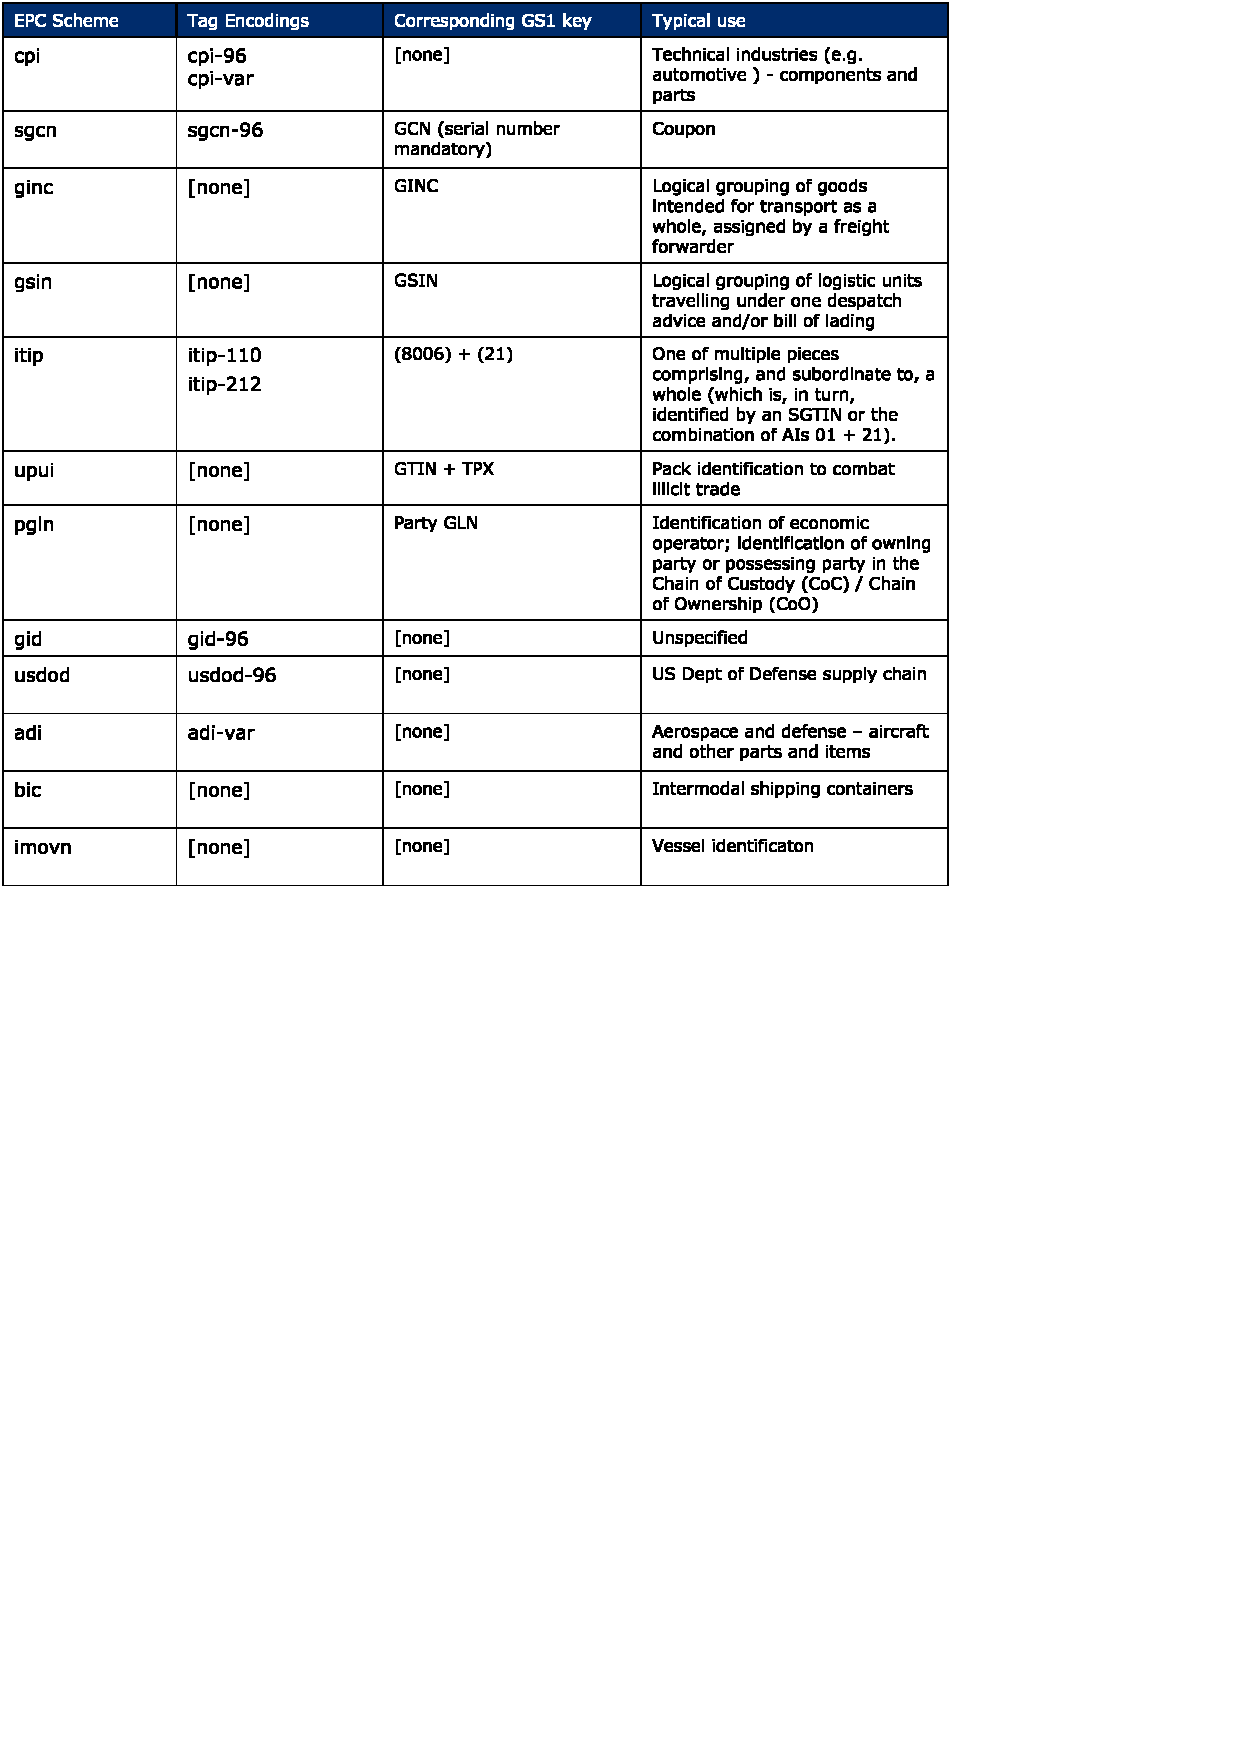
\includegraphics[width=\textwidth]{./figs/02-state-of-the-art/epcschemes2.pdf}
    \caption[\ac{epc} Schemes and Corresponding GS1 keys Part 2]{\ac{epc} Schemes and Corresponding GS1 keys Part 2~\cite{EPCTagData}}
\end{table}

\clearpage

\section{\ac{llrp} Messages} \label{anx:llrpmessages}
\begin{table}[!ht]
    \centering
    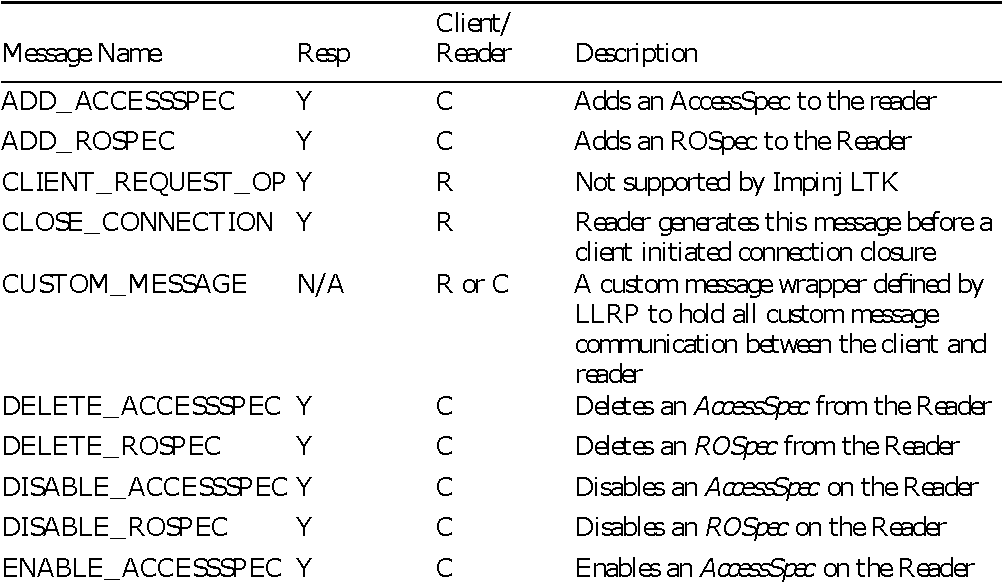
\includegraphics[width=\textwidth]{./figs/02-state-of-the-art/table_llrpmessages_1.pdf}
    \caption[\ac{llrp} Messages (except for responses) Part 1]{\ac{llrp} Messages (except for responses) Part 1~\cite{ImpinjLTKProgrammers}} 
    \label{tab:llrpmessages1}
\end{table}


\begin{table}
    \centering
    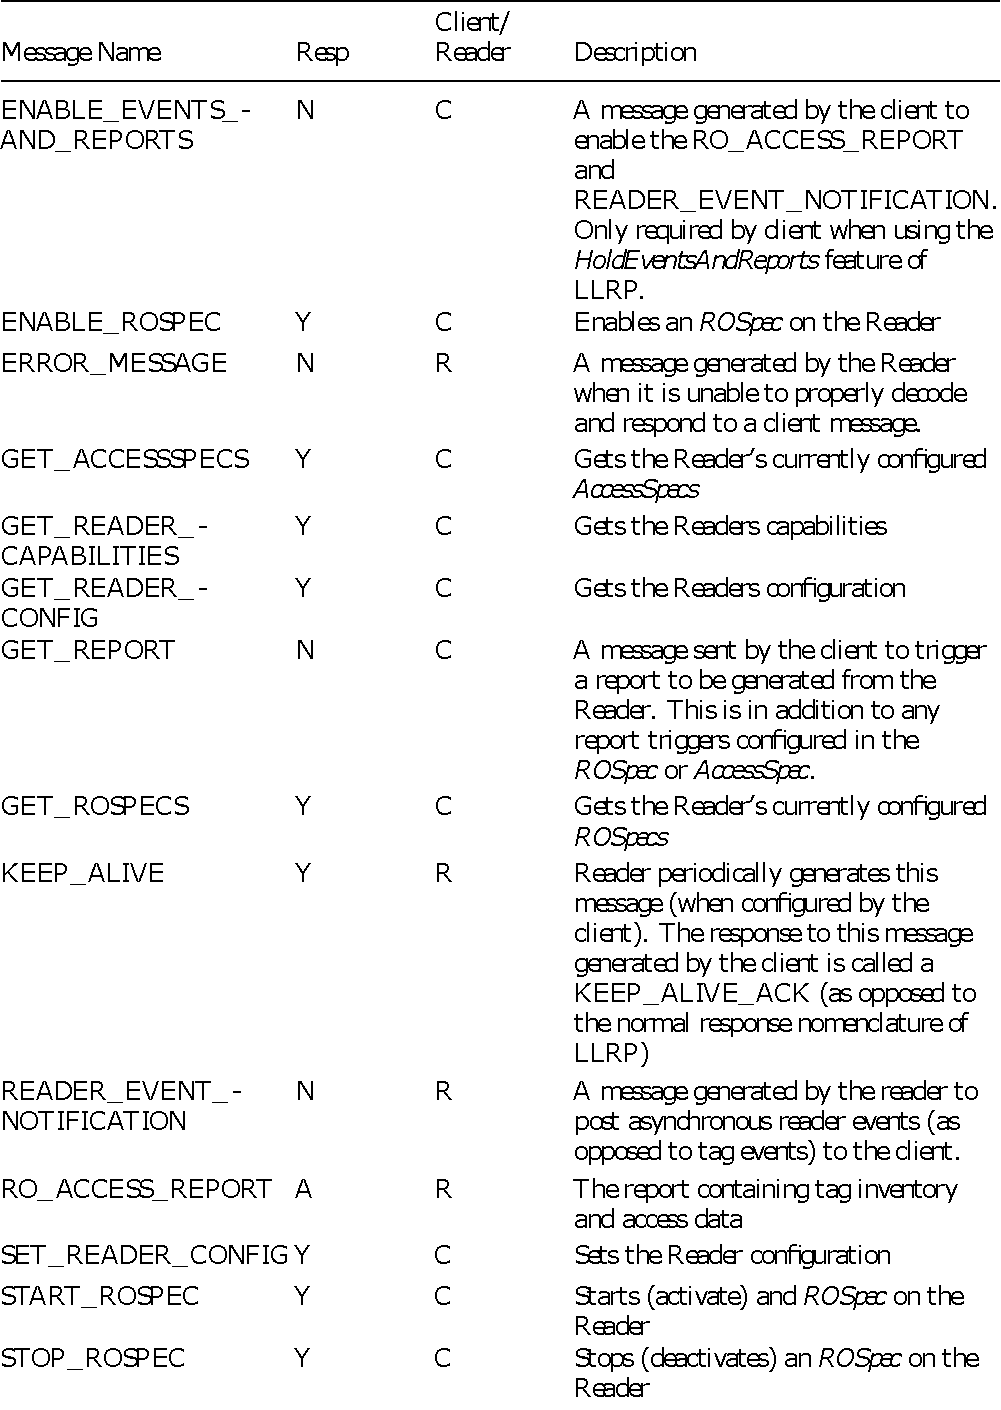
\includegraphics[width=\textwidth]{./figs/02-state-of-the-art/table_llrpmessages_2.pdf}
    \caption[\ac{llrp} Messages (except for responses) Part 2]{\ac{llrp} Messages (except for responses) Part 2~\cite{ImpinjLTKProgrammers}} 
    \label{tab:llrpmessages2}
\end{table}

\clearpage

\section{Production Docker Compose file} \label{apx:composefile}
\inputminted[linenos, breaklines, frame=single]{yaml}{./code/docker-compose-production.yml}

\clearpage

\section{Octane SDK Reader Configuration Program} \label{apx:octanereaderconfig}
\inputminted[linenos, breaklines, frame=single]{java}{./code/App.java}

\clearpage

\section{\acs{xml} Reader Configuration Message Files} \label{apx:xmlreaderconfig}
\inputminted[linenos, breaklines, frame=single]{xml}{./code/SET_READER_CONFIG.xml}
\pagebreak
\inputminted[linenos, breaklines, frame=single]{xml}{./code/ADD_ROSPEC.xml}

\clearpage

\section{Reader Capabilities from \textit{GET\_READER\_CAPABILITIES\_RESPONSE} message}
\label{apx:readercapabilities}
\inputminted[linenos, breaklines, frame=single]{xml}{./code/GET_READER_CAPABILITIES_RESPONSE.xml}

\clearpage

\section{Impinj Readers Search Modes}
\label{apx:searchmodes}
\begin{table}[!ht]
    \centering
    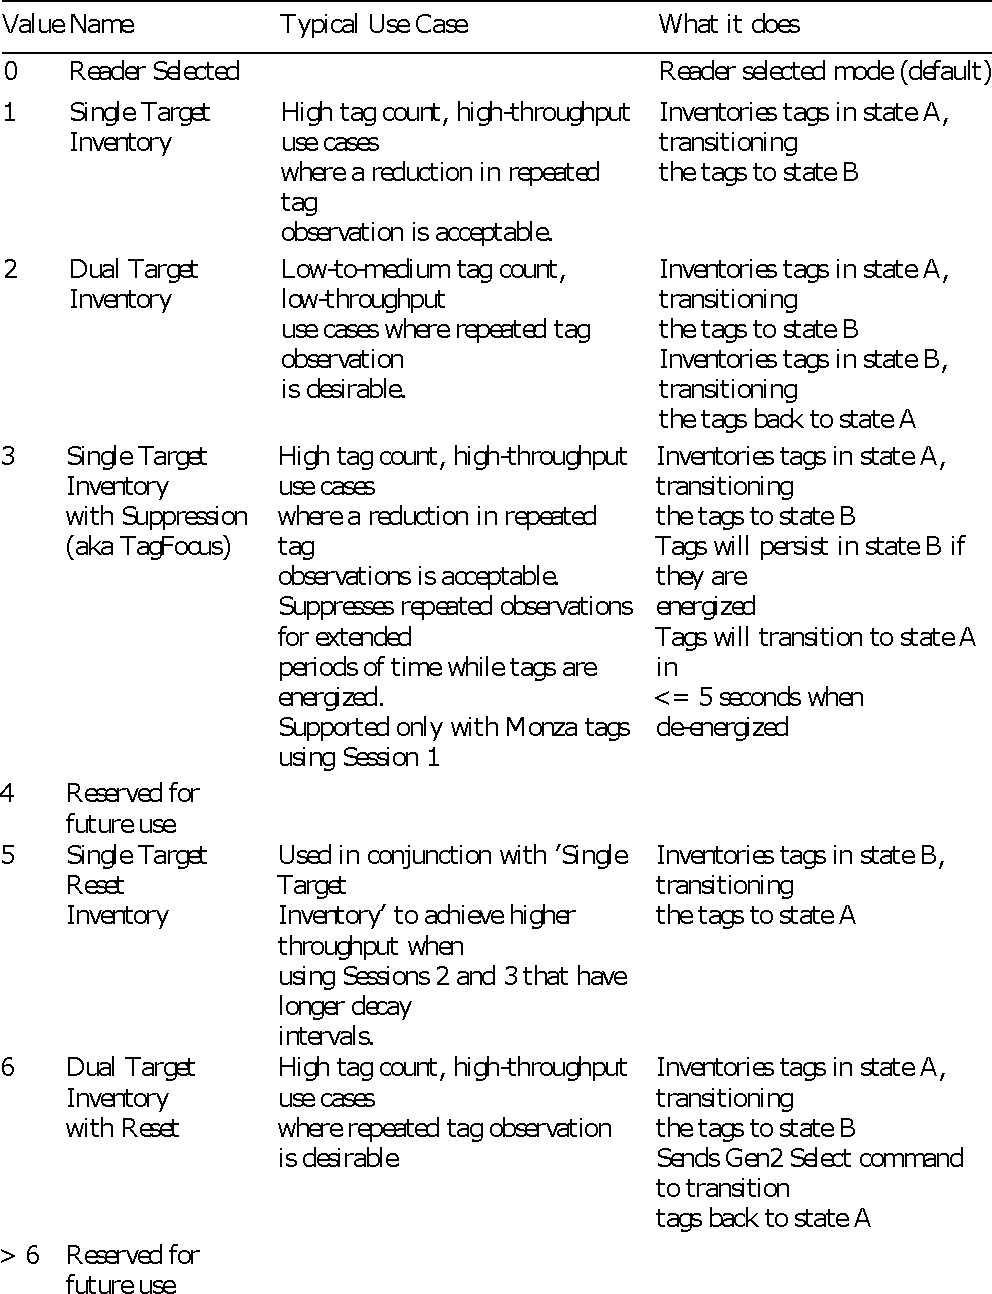
\includegraphics[width=\textwidth]{./figs/searchmodes.pdf}
    \caption{Impinj Readers Search Modes~\cite{ImpinjOctaneLLRP}} 
\end{table}

\end{appendices}